%======================================================================
%	
%	 __  __       _         ______ _ _      
%	|  \/  |     (_)       |  ____(_) |     
%	| \  / | __ _ _ _ __   | |__   _| | ___ 
%	| |\/| |/ _` | | '_ \  |  __| | | |/ _ \
%	| |  | | (_| | | | | | | |    | | |  __/
%	|_|  |_|\__,_|_|_| |_| |_|    |_|_|\___|
%
%----------------------------------------------------------------------
% Descripton : Main File to compose the resulting PDF
%======================================================================
%\pdfobjcompresslevel=0
\pdfminorversion=7
\pdfinclusioncopyfonts=1
\documentclass[
				ngerman             % neue deutsche Rechtschreibung
				,a4paper            % Papiergrösse
				,twoside            % Zweiseitiger Druck (rechts/links)
				% ,10pt             % Schriftgrösse
				,11pt
				% ,12pt
				,pdftex
				%  ,disable         % Todo-Markierungen auschalten
				,notitlepage		% Thanks abstract... preventing it from removing pageNumber
				]{report}

%————————————————————————————————————————————————————————————————————————————
%					Import aller Konfigurationen
%————————————————————————————————————————————————————————————————————————————
\usepackage{./config/DHBW/bericht}
\usepackage{./config/PaketeProjektarbeit} % <- spezifische Pakete für die Projektarbeit
\usepackage{./config/Pakete}
\usepackage{./config/Befehle}
\usepackage{./config/Layout}
\usepackage{./config/Styles}
%Wenn PDF/A-1B gewünscht .. Achtung am besten nochmal mit veraPDF testen!
\usepackage{./config/PDFStandard}

%————————————————————————————————————————————————————————————————————————————
%					Variablen deklarieren
%————————————————————————————————————————————————————————————————————————————
\include{./config/Variables}

%————————————————————————————————————————————————————————————————————————————
%					Informationen ausfüllen
%————————————————————————————————————————————————————————————————————————————
%======================================================================
%	
%	_____        __                           _   _             
%  |_   _|      / _|                         | | (_)            
%	 | |  _ __ | |_ ___  _ __ _ __ ___   __ _| |_ _  ___  _ __  
%    | | | '_ \|  _/ _ \| '__| '_ ` _ \ / _` | __| |/ _ \| '_ \ 
%	_| |_| | | | || (_) | |  | | | | | | (_| | |_| | (_) | | | |
%  |_____|_| |_|_| \___/|_|  |_| |_| |_|\__,_|\__|_|\___/|_| |_|
%
%----------------------------------------------------------------------
% Descripton : File with all Information about the Document
%======================================================================

\newcommand{\Autor}{Nico Holzhäuser}
\newcommand{\MatrikelNummer}{...TBD...}
\newcommand{\Kursbezeichnung}{TINF19B4}

\newcommand{\FirmenLogoDeckblatt}{
\includegraphics[width=2.5cm]{./config/layout/WhiskeyOClock}}

% Falls es kein Firmenlogo gibt:
%  \newcommand{\FirmenLogoDeckblatt}{}

\newcommand{\BetreuerDHBW}{Mirko Dostmann}

%%%%%%%%%%%%%%%%%%%%%%%%%%%%%%%%%%%%%%%%%%%%%%%%%%%%%%%%%%%%%%%%%%%%%%%%%%%%%%%%%%%%%

% Wird auf dem Deckblatt und in der Erklärung benutzt:
%\newcommand{\Was}{Projekt-/Studien-/Bachelorarbeit}
%\newcommand{\Was}{Projektrarbeit}
%\newcommand{\Was}{Studienarbeit}
%\newcommand{\Was}{Bachleorarbeit}
\newcommand{\Was}{Programmentwurf}

%%%%%%%%%%%%%%%%%%%%%%%%%%%%%%%%%%%%%%%%%%%%%%%%%%%%%%%%%%%%%%%%%%%%%%%%%%%%%%%%%%%%%

\newcommand{\Titel}{Whiskey 'o clock}
\newcommand{\AbgabeDatum}{5. Mai 2022}

\newcommand{\Dauer}{5. \& 6. Semester}

% \newcommand{\Abschluss}{Bachelor of Engineering}
\newcommand{\Abschluss}{Bachelor of Science}

%\newcommand{\Studiengang}{Informatik / Informationstechnik}
\newcommand{\Studiengang}{Informatik / Angewandte Informatik}
\include{./config/HyperrefSetup}


%————————————————————————————————————————————————————————————————————————————
%					Sonstige Einstellungen
%————————————————————————————————————————————————————————————————————————————
\bibliography{./directories/bibliography}
\loadglsentries{./directories/glossary}
\makeglossaries

%————————————————————————————————————————————————————————————————————————————
%					Einstellungen
%————————————————————————————————————————————————————————————————————————————
% Debug auf true setzen, hierbei wird der Changelog hinzugefügt, und keine Doppelseitenumbrüche gemacht (Zum drucken -> false)
% Bitte zum drucken oben in der Präambel auch auf Doppelseite schalten!
\setboolean{DEBUG}{true}
% Soll eine Erklärung eigefügt werden ?
\setboolean{ERKLAERUNG}{false}
%Soll das Abstract eingefügt werden ?
\setboolean{ABSTRACT}{false}
%Soll ne Trennlinie im Inhaltsverzeichnis eingefügt werden, vor Verzeichnissen, dem Inhalt und dem Anhang
\setboolean{TRENNSTRICHE}{true}
%Setzt ein Watermark
\setboolean{WATERMARK}{false}
%Dokumentenverzeichnis generieren ?

%————————————————————————————————————————————————————————————————————————————
%					Watermark
%————————————————————————————————————————————————————————————————————————————
\ifthenelse{\boolean{WATERMARK}}{\usepackage{draftwatermark}}{}
\ifthenelse{\boolean{WATERMARK}}{\SetWatermarkText{Entwurf}}{}

%————————————————————————————————————————————————————————————————————————————
%									Anfang Dokument
%————————————————————————————————————————————————————————————————————————————
\begin{document}
	% Wer keine Seitenzahlen braucht bis zum TOC einfach das Pagenumbering auf gobble und an der Stelle an der die Seitenzählung beginnen soll roman einfügen
	\pagenumbering{gobble}
	\pagestyle{plain}
	
	%—————————————————————————————————————————————————————————————————————————
	%								Deckseite
	%—————————————————————————————————————————————————————————————————————————
	\begin{titlepage}
		\include{./pages/orga/titlepage}
	\end{titlepage}

	% Ab hier beginnt die Seitenzählung für den Prefix in kleinen römischen Zahlen
	% Erste Seite nach der Titelseite
	\pagenumbering{roman}
	\setcounter{page}{2}
	\ifthenelse{\boolean{DEBUG}}{}{\cleardoublepage}
	
	%—————————————————————————————————————————————————————————————————————————
	%								Erklärung
	%—————————————————————————————————————————————————————————————————————————
	\ifthenelse{\boolean{ERKLAERUNG}}{\phantomsection}{}
	\ifthenelse{\boolean{ERKLAERUNG}}{\input{./pages/orga/erklaerung.tex}}{}
	\ifthenelse{\boolean{ERKLAERUNG}}{\addcontentsline{toc}{chapter}{Erklärung}}{}
	\ifthenelse{\boolean{DEBUG}}{}{\cleardoublepage}
	
	%—————————————————————————————————————————————————————————————————————————
	%								Abstract
	%—————————————————————————————————————————————————————————————————————————
	\ifthenelse{\boolean{ABSTRACT}}{\phantomsection}{}
	\ifthenelse{\boolean{ABSTRACT}}{\include{./pages/content/abstract}}{}
	\ifthenelse{\boolean{DEBUG}}{}{\cleardoublepage}
	
	%—————————————————————————————————————————————————————————————————————————
	%							Inhaltsverzeichnis
	%—————————————————————————————————————————————————————————————————————————
	\setcounter{tocdepth}{1}% Allow only \chapter in ToC
	\ifthenelse{\boolean{DEBUG}}{}{\cleardoublepage}
	
	\phantomsection
	\addcontentsline{toc}{chapter}{Inhaltsverzeichnis}
	\tableofcontents           % Inhaltsverzeichnis hier ausgeben
	\ifthenelse{\boolean{DEBUG}}{\newpage}{\cleardoublepage}
	
	\phantomsection
	\listoffigures             % Liste der Abbildungen
	\addcontentsline{toc}{chapter}{Abbildungsverzeichnis}
	\ifthenelse{\boolean{DEBUG}}{\newpage}{\cleardoublepage}
	
	\phantomsection
	\lstlistoflistings         % Liste der Codeschnipsel
	\addcontentsline{toc}{chapter}{Codeverzeichnis}
	\ifthenelse{\boolean{DEBUG}}{\newpage}{\cleardoublepage}
	
	\phantomsection
	\ifthenelse{\boolean{TRENNSTRICHE}}{\addtocontents{toc}{\protect\mbox{}\protect\hrulefill\par}}{}
	%======================================================================
%                                              
%	    /\                                        
%	   /  \   ___ _ __ ___  _ __  _   _ _ __ ___  
%	  / /\ \ / __| '__/ _ \| '_ \| | | | '_ ` _ \ 
%	 / ____ \ (__| | | (_) | | | | |_| | | | | | |
%	/_/    \_\___|_|  \___/|_| |_|\__, |_| |_| |_|
% 	                              __/ |          
%	                              |___/             
%
%----------------------------------------------------------------------
% Author : Nico Holzhäuser
% Descripton : Cover Page
%======================================================================

\chapter*{Abkürzungsverzeichnis} % chapter*{..} --> keine Nummer, kein "Kapitel"
						         % Nicht ins Inhaltsverzeichnis
\addcontentsline{toc}{chapter}{Abkürzungsverzeichnis}   % Damit das doch ins Inhaltsverzeichnis kommt

% Hier werden die Abkürzungen definiert
% 1-10 nur damit der Abstand default auf diese Länge gesetzt wird
\begin{acronym}[12345678910]
  	%\acro{Name}{Darstellung der Abkürzung}{Langform der Abkürzung}
  	\acro{API}[API]{Application Programming Interface}
  	\acro{DDD}[DDD]{Domain Driven Design}
	\acro{DHBW}[DHBW]{Duale Hochschule Baden-Württemberg}
	\acro{IDE}[IDE]{Integrated Development Environment}
	\acro{UML}[UML]{Unified Modeling Language}
	\acro{UC}[UC]{Use Case}


	% Folgendes benutzen, wenn der Plural einer Abk. benöigt wird
	% \newacroplural{Name}{Darstellung der Abkürzung}{Langform der Abkürzung}
	\newacroplural{Abk}[Abk-en]{Abkürzungen}

	% Wenn neicht benutzt, erscheint diese Abk. nicht in der Liste
	\acro{NUA}[]{Not Used Acronym}
	
\end{acronym}
 %Acronyms

	\ifthenelse{\boolean{DEBUG}}{\newpage}{\cleardoublepage}
		
	
	%—————————————————————————————————————————————————————————————————————————
	%								Inhalt
	%—————————————————————————————————————————————————————————————————————————
	%Hauptteil normale arabische Zählung, beginnend bei 1 und alten Pagestyle wiederherstellen!
	\pagenumbering{arabic} 
	\setcounter{page}{1}
	\pagestyle{headings} %<- Pagestyle reset 
	
	%%%%%%%%%%%%%%%%%%%%%%%%%%%%%%%%%%%%%%%%%%%%%%%%%%%%%%%%%%%%%%%%%%%%%%%%%%%%%%%
%% Descr:       Vorlage für Berichte der DHBW-Karlsruhe
%% Author:      Prof. Dr. Jürgen Vollmer, vollmer@dhbw-karlsruhe.de
%% Modified :	Nico Holzhäuser, TINF19B4
%% -*- coding: utf-8 -*-
%%%%%%%%%%%%%%%%%%%%%%%%%%%%%%%%%%%%%%%%%%%%%%%%%%%%%%%%%%%%%%%%%%%%%%%%%%%%%%%

\chapter{Domain Driven Design}
	

	\section{Ubiquitous Language}
	Die \hk{ubiquitous language} ist ein Begriff, den \citeauthor{evans2004ddd} in seinem Buch \citetitle{evans2004ddd} eingeführt hat. Dieser Begriffs beschreibt die allgegenwärtige Sprache, die von Softwareentwickler*innen und Fachexpert*innen gemeinsam gesprochen wird \cite{ubiquitousLanguage.entwicklerDE}. Sie soll der Basis für die Entwicklung des Softwaremodells sein.
	
		\subsection{Analyse der Ubiquitous Language}
		In diesem Projekt ist die \hk{ubiquitous language} relativ einfach gehalten, da die Fachdomäne überschaubar ist. Aufgrund dieser beschränkten Problemdomäne sollten keine schwerwiegenden Kommunikationsprobleme in der gemeinsamen Sprache auftreten. Jedoch ist es auch hier wichtig, bestimmte Thematiken und Objekttypen exakt zu spezifizieren um Problemen direkt vor deren Entstehung entgegenzuwirken.
		
		\begin{table}[ht]
			\begin{adjustbox}{width=1\textwidth}
				\begin{tabular}{|l|c|}
					\hline
					\multicolumn{2}{|c|}{Ubiquitous Language} \\
					\hline
					Ubiquitous Language			&		\hk{normale} Definition \\
					\hline
					\hline
					Country						& 		Entität für das Herkunftsland einer Flasche \\
					\hline
					Manufacturer				& 		Hersteller / Abfüller der Flasche \\
					\hline
					Whiskeyflasche				&		Kleinste Entität des Systems. Einfach nur eine schöne, meist teure, Flasche Whiskey \\
					\hline
					Serie						&		0 .. n Whiskeyflaschen bilden zusammen eine Serie. Diese haben meist einen gemeinsamen Faktor, wie z.B. die Herkunft \\
					\hline
				\end{tabular}
			\end{adjustbox}
		\end{table}
	
			\subsubsection{Verbindungen zwischen den Objekten \cite{projektantrag.holzhaeuser}}
			Die Grundlage sollen einezelne Whiskeyflaschen-Objekte bilden. Diese werden durch ihre \textbf{Herkunft, das Alter, den Kaufpreis, die Sorte und den aktuellen Status} definiert. Hierbei müssen bei einer Objektanlage zwingend ein \textbf{label} und eine \textbf{Manufacture} definiert werden. Diese Objekte können als \textbf{einzelne Flasche oder als Teil einer Serie} angelegt werden. Hierbei soll ein Objekt nur Teil \textbf{einer oder keiner} Serie sein können. Außerdem sollen Objekte als \textcolor{gray}{'Favoriten'},\textcolor{gray}{'Unverkäufliche'} bzw. als \textcolor{gray}{im Angebot zum Verkauf} gekennzeichnet werden können. Hierbei können \textcolor{red}{favorisierte} sowie \textcolor{red}{unverkäufliche} Flaschen nicht in den Status \textcolor{gray}{'zum Verkauf'} wechseln ohne vorher die entsprechenden Kennzeichnungen zu entfernen.
			
			Eine Serie besteht aus einer Anzahl an Objekten > 1. Hierbei können verschiedene Flaschen zu einer Serie zusammengefasst werden. Eine Serie benötigt immer zwingend eine Bezeichnung und eine Menge an zugehörigen Objekten. Sind alle Objekte in einer Serie mit dem Status 'zum Verkauf' gekennzeichnet kann die ganze Serie '**zum Verkauf**' angeboten werden. Werden Objekte gelöscht so soll die Serie automatisch angepasst, und bei einem Inhalt von weniger als zwei Flaschen gelöscht werden.
			
			Objekte sowie können des weiteren gelöscht, sowie verändert werden.
	
		\subsection{Probleme bei der Ubiquitous Language \& deren Lösung \cite{ubiquitousLanguage.medium}}
		\begin{itemize}
			\item Übersetzen von komplexen Sachinhalten in einfache Sprache
			\begin{itemize}
				\item[] → Durch Wortdefinitionen eliminiert
			\end{itemize}
			\item Unterschiedliche Bezeichnungen für ein und das Selbe
			\begin{itemize}
				\item[] → Begriffe aus dem Definitionspool verwenden
			\end{itemize}
			\item Abstraktion der technischen Sachverhalte für die Domain Experten
			\begin{itemize}
				\item[] → Klar und deutliche Definitionen im Team und ständige Weiterentwicklung der Ubiquitous Language
			\end{itemize}
			\item Keine Rücksichtnahme der Domain Experten bei der Entwicklung des technischen Modells
			\begin{itemize}
				\item[] → Mit einbeziehen alles Parteien für das bestmögliche Ergebnis
			\end{itemize}
		\end{itemize}
	
	\section{Analyse und Begründung der verwendeten Muster}
		
		\subsection{Analyse}
		Eine komplette Übersicht des \acl{DDD} ist in Anhang in \cref{a.1.ddd} beigefügt.
			
			\subsubsection{Value Objects \cite{valueObjects.medium}} \label{1.va}
			Das Value Object ist ein in der Softwareentwicklung häufig eingesetztes Entwurfsmuster. Wertobjekte(engl. \hk{Value Objects}) sind unveränderbare Objekte, die einen speziellen Wert repräsentieren. Soll der Wert geändert werden, so muss ein neues Wertobjekt erzeugt werden.
			
			\subsubsection{Entities \cite{domainModell.microsoft}} \label{1.ent}
			Entitäten stellen im Domänemodell Objekte da, welche nicht nur durch die darin enthaltenen Attribute definiert, sondern primär durch ihre Identität, Kontinuität und Persistenz im Laufe der Zeit definiert werden. Entitäten sind im Domänenmodell sehr wichtig, da sie die Basis eines Modells darstellen.
			
			\subsubsection{Aggregates \cite{domainModell.microsoft}} \label{1.aggregates}
			Ein Aggregat umfasst mindestens eine Entität: den sogenannten Aggregatstamm, der auch als Stammentität oder primäre Entität bezeichnet wird. Darüber hinaus kann es über mehrere untergeordnete Entitäten und Wertobjekte verfügen, wobei alle Entitäten und Objekte zusammenarbeiten, um erforderliche Verhaltensweisen und Transaktionen zu implementieren. \cref{a.1.aggregate}
			
			\subsubsection{Repositories \cite{repository.medium}}
			Ein Repository vermittelt zwischen der Domänen- und der Datenzuordnungsebene mithilfe einer sammlungsähnlichen Schnittstelle für den Zugriff auf Domänenobjekte. Hierbei kann die Anwendung einfach vorhandene Entitäten aus der Persistenzebene laden, speichern, updaten oder löschen.
			
			\subsubsection{Domain Service \cite{domainService.gorodinski}}
			Eric Evans beschreibt in seinem Buch \citetitle{evans2004ddd} einen Domänen Service wie folgt : 
			\begin{displayquote}
				When a significant process or transformation in the domain is not a natural responsibility of an ENTITY or VALUE OBJECT, add an operation to the model as standalone interface declared as a SERVICE. Define the interface in terms of the language of the model and make sure the operation name is part of the UBIQUITOUS LANGUAGE. Make the SERVICE stateless.
			\end{displayquote}
			Hierbei ist grob gesagt, dass ein signifikanter Prozess oder eine Transformation, die über die Verantwortung einer Entität hinaus geht, als eine eigenständige Operation des Modells als Interface mit dem Namen \hk{Service} hinzugefügt werden muss. Somit beschreibt ein Service einen Prozess, der über die Verantwortung einer Entität oder eines Wertobjektes hinaus geht.
		
		\subsection{Begründung}
		
			\subsubsection{Value Objects}
			In diesem Projekt sollen Wertobjekte dazu dienen, die Übertragung zwischen Backend und Frontend zu gewährleisten. Meist werden Sie für Read-,Update- oder Modifizierungsaufrufe verwendet. Hierbei sind diese \hk{DTO} Objekte unveränderlich und haben meist die Inhalte einer Entität. So können Entitäten in einer Serialisierten Form ausgetauscht werden.
			
			\subsubsection{Entities}
			In diesem Projekt sind vier Entitäten vorhanden, die die Basis des Domänenmodells bilden vorhanden :
			\begin{itemize}
				\item \class{Country} - Land
				\item \class{Manufacturer} - Hersteller/Abfüller
				\item \class{Bottle} - Flasche
				\item \class{Serie} - Flaschenserie
			\end{itemize}
			Diese werden durch ihre Identität selbst beschriebene, werden persistiert und haben veränderliche Attribute.
			
			\subsubsection{Aggregates}
			Aggregate sind in diesem Projekt im eigentlichen Sinne nicht vorhanden. Jedoch sind nach der Definition in \cref{1.aggregates} auch einzelne Entitäten ein Aggregatstamm und somit ein Aggregate im jeweiligen Bereich. Folgen wir diesem Prinzip gibt es in diesem Projekt \textbf{vier} Aggregate.
			
			\subsubsection{Repositories}
			In diesem Projekt sind Repositories im Backend zu finden. Hierbei werden sie durch Implementierungen des Interfaces \interface{JpaRepository<Object,PrimaryKey>} umgesetzt. Mit der Hilfe von Hibernate wird so die Persistierungsschicht mit der Applikationsschicht verbunden und Methoden geschaffen, um Objekte aus der Datenbasis zu filtern.
			
			\subsubsection{Domain Service}
			Service's finden in diesem Projekt ebenfalls im Backend ihre Anwendung. Hierbei wird die Logik in sogenannte Services ausgelagert, die bestimmte Entitäten oder Beziehungen anhand eines \ac{UC} bearbeiten. Hierbei sind in Spring Boot oft die \ac{API} Aufrufe einzelne gekapselte Logiken, welche durch einen entsprechenden Serviceaufruf umgesetzt werden. \\ 
			Des weiteren sind Security oder Transaktionale Komponenten denkbare Services für eine Spring Anwendung.
	\ifthenelse{\boolean{DEBUG}}{}{\cleardoublepage}
	
	%%%%%%%%%%%%%%%%%%%%%%%%%%%%%%%%%%%%%%%%%%%%%%%%%%%%%%%%%%%%%%%%%%%%%%%%%%%%%%%
%% Descr:       Vorlage für Berichte der DHBW-Karlsruhe
%% Author:      Prof. Dr. Jürgen Vollmer, vollmer@dhbw-karlsruhe.de
%% Modified :	Nico Holzhäuser, TINF19B4
%% -*- coding: utf-8 -*-
%%%%%%%%%%%%%%%%%%%%%%%%%%%%%%%%%%%%%%%%%%%%%%%%%%%%%%%%%%%%%%%%%%%%%%%%%%%%%%%

\chapter{Clean Architecture}

	\section{Schichtenarchitektur}
	Im \cite{} \cref{a.2.cleanArchitecture}
	
	\subsection{Planung}
	
	\subsection{Entscheidung anhand von Kriterien}
	\ifthenelse{\boolean{DEBUG}}{}{\cleardoublepage}
	
	%%%%%%%%%%%%%%%%%%%%%%%%%%%%%%%%%%%%%%%%%%%%%%%%%%%%%%%%%%%%%%%%%%%%%%%%%%%%%%%
%% Descr:       Vorlage für Berichte der DHBW-Karlsruhe
%% Author:      Prof. Dr. Jürgen Vollmer, vollmer@dhbw-karlsruhe.de
%% Modified :	Nico Holzhäuser, TINF19B4
%% -*- coding: utf-8 -*-
%%%%%%%%%%%%%%%%%%%%%%%%%%%%%%%%%%%%%%%%%%%%%%%%%%%%%%%%%%%%%%%%%%%%%%%%%%%%%%%

\chapter{Programming Principles}

	\section{SOLID \cite{solid.servinc}}
	Hinter der Bezeichnung \hk{SOLID} stehen fünf Prinzipien
	\begin{itemize}
		\item \textbf{SRP} Single-Responsibility-Prinzip
		\item \textbf{OCP} Open-Closed-Prinzip
		\item \textbf{LSP} Liskov’sche Substitutions-Prinzip
		\item \textbf{ISP} Interface-Segregation-Prinzip
		\item \textbf{DIP} Dependency-Inversion-Prinzip
	\end{itemize}
		\subsection{Single-Responsibility-Prinzip}
		Dieses Prinzip findet zum Beispiel in den Repositor's seinen Nutzen. Dieses haben nur eine Funktion, die Schnittstelle zur Datenbank darzustellen. Dies ist ihr einziger definierter Aufgabenbereich.
		
		\subsection{Open-Closed-Prinzip}
		Das Open-Closed-Prinzip besagt, dass Objekte einfach erweiterbar sind und die bestehende Logik nicht in ihren fundamentalen Bestandteilen modifiziert werden muss. \\
		Ein Beispiel ist hier der \hk{BottleApplicationService}, der mit Hilfe der Klasse \hk{BottleBooleanType} eine Unterscheidung der \hk{checkbaren} Boolean Werte ermöglicht. Kommt hier ein neuer hinzu muss nur das Enum erweitert werden und im Switch-Case ein neuer Fall implementiert werden.
		
		\subsection{Liskov’sche Substitutions-Prinzip}
		Das Liskov'sche Substitutions Prinzip findet keine Anwendung, da keine Vererbung implementiert wurde.
		
		\subsection{Interface-Segregation-Prinzip}
		Das Interface-Segregation-Prinzip besagt, dass Entwickler nicht dazu gezwungen werden sollen Teile von Schnittstellen zu implementieren, die später nicht verwendet werden. Prinzipiell wurde dieses Prinzip, durch den Aufbau der Interfaces in verschiedene Zuständigkeitsbereiche, direkt umgesetzt und die Interfaces müssen nicht weiter aufgeteilt werden.
		
		\subsection{Dependency-Inversion-Prinzip}
		Das Dependency-Inversion-Prinzip besagt, dass Systeme am flexibelsten sind, wenn Codeabhängigkeiten ausschließlich auf Abstraktion beziehen, statt auf Konkretionen. In Java soll sich hier bei der Nutzung von import nur auf abstrakte Quellmodule bezogen werden, wie z.B Schnittstellen, abstrakte Klassen oder Module, die jede andere Form der Abstraktion gewährleisten. \\
		In der Praxis ist diese Regel aber kaum umsetzbar, da Softwaresysteme auch von konkreten Entitäten abhängig sind. Im groben folgen die Module der \cref{2.cleanArchitecture} diesem Prinzip, da nur Module von höhren Schichten die Interfaces aus den niedrigeren Schichten implementieren. Somit liegen die Regeln in der inneren Schicht, wohingegen die Implementierung in den äußeren Schichten vorgenommen werden.

	\section{GRASP (insb. Kopplung/Kohäsion)}
	Unter der Bezeichnung \hk{GRASP} (\textbf{G}eneral \textbf{R}esponsibility \textbf{A}ssignment \textbf{S}oftware \textbf{P}rinciples) versteht man neun grundlegende Muster
	\begin{enumerate}
		\item Controller(engl. Controller)
		\item Ersteller (engl. Creator)
		\item Indirektion (engl. Indirection)
		\item Informationsexperte (engl. Information expert)
		\item Hohe Kohäsion (engl. High cohesion)
		\item Wenig Koppelnd (engl. Low coupling)
		\item Polymorphie (engl. Polymorphism)
		\item (engl. Protected variations)
		\item (engl. Pure fabrication)
	\end{enumerate}
	Im weiteren werden die \textbf{Prinzipien 5,6} genauer betrachtet.
		
	\newpage
		
		\subsection{Analyse}
		\begin{enumerate}
			\item Bei Spring werden die Events (in unserem Fall API Calls) durch sogeannte Controller behandelt. Diese liegen im \modul{0 - Plugins} im \package{de.dhbw.ase.plugin.rest}
			\item -
			\item -
			\item -
			\item Näher in \cref{3.highCohesion} behandelt
			\item Näher in \cref{3.lowCoupling} behandelt
			\item -
			\item -
			\item -
 		\end{enumerate}
	
			\subsection{High cohesion \cite{kohaesion.google}} \label{3.highCohesion}
			Das Prinzip \hk{Hohe Kohäsion} (engl. high cohension) besagt, dass darauf geachtet werden soll, dass diese Klasse nicht mehrere Verantwortlichkeiten in sich trägt. Die Kohäsion ist ein Maß für den logischen Zusammenhang der Daten und Methoden der Klasse. So sollten keine Verantwortlichkeiten und Aufgaben \textbf{in} einer Klasse vermischt werden. \\
			Dieses Prinzip wurde im ganzen Projekt umgesetzt. Einige Beispiele hierfür sind die JPA-Repository's, die nur Kenntnisse von ihrer Anbindung an die Datenbasis haben und keine weiteren Verbindungen zu anderen Objekten benötigen, oder die Controller, die nur Events entgegennehmen und sie entsprechend mit Hilfe der Services verarbeiten. Hier ist jeweils eine hohe Kohäsion gegeben.
			
			\subsection{Low coupling \cite{kohaesion.google}} \label{3.lowCoupling}
			Das Prinzip \hk{wenig Kopplung} (engl. low coupling) besagt, dass möglichst wenig Abhängigkeiten zwischen den Komponenten bestehen sollte. Die einzelnen Klassen/Objekte/Module sollten möglichst wenig voneinander wissen. Das Ziel ist die Abhängigkeiten zwischen einzelnen Klassen/Objekte/Module so gering wie möglich zu halten. \\
			Dieses Prinzip wurde im ganzen Projekt umgesetzt. Ein Beispiel ist, dass z.B. der CountryApplicationService kein wissen über andere Repoistory's als das \hk{CountryRepository} benötigt. Hier herscht also \hk{low coupling}. Im Gegenzug benötigt der \hk{BottleApplicationService} drei verschiedene Repository's, was eine hohe Kopplung mit sich bringt.
			
		\subsection{Schlussfolgerung}
		Prinzipiell geht die Kohäsion mit der Kopplung einher. Umso mehr Verantwortlichkeiten und Teilaufgaben in andere Klassen ausgelagert werden, umso höher wird die Kohäsion der Ursprungsklasse, da hier eine Spezialisierung stattfindet. Im gleichen Schritt nimmt ebenfalls die Kopplung zu, da die Ursprungsklasse von mehreren Unterklassen abhängig ist. Hierbei gilt es ein gesundes Mittelmaß zu finden und eine überlegte Trennung durchzuführen. Generell gilt jedoch die Kopplung unter Klassen gering und damit die Kohäsion der Klassen hoch zu halten.
		
		
		
	\section{DRY}
	Das Programmierprinzip \hk{DRY}, dt. für \hk{wiederholde dich nicht} (engl. \textbf{D}on't \textbf{R}epeat \textbf{Y}ourself), steht für ein Prinzip in der Programmierung. Hierbei sollen Redundanzen vermieden bzw. beseitigt werden. Es ist ein fundamentales Prinzip von Clean Code, dass von Programmieren wie folgt definiert wird :
	\par Every piece of knowledge must have a single, unambiguous, authoritative representation within a system. \cite{dry.thevaluable}
	\\
		\subsection{Analyse}
		DRY ist ein grundlegendes Prinzip in der Programmierung und prinzipiell überall im Projekt zu finden. So wurde Beispielsweise die Konstruktoren der \class{Bottle} ineinander verzahnt, um die Zuweisung lediglich einmal entwickeln zu müssen. Ebenso wurden Mapper geschaffen, um die Umwandlungslogik zentral an einem Ort abzulegen und nicht an jeder Stelle, an der diese Logik benötigt wird eine eigene Implementierung zu benötigen.
		
		\subsection{Begründung}
		Die Anwendung der \hk{DRY} Prinzipien bringt einige Vorteile mit sich. So ist weniger Code generell besser da es Zeit und Aufwand mit sich bringt diesen Code zu warten. Außerdem werden Fehler durch weniger Code vermieden, da schlichtweg weniger Platz vorhanden ist um Fehler zu machen. Des weiteren hilft es dabei, wenn bestimmte Logiken ausgelagert werden, wie z.B die Mapper Logiken da diese an vielen Stellen in der Anwendung verwendet und dadurch wiederverwendet werden können. Zuletzt muss, wenn ein Logikfehler auftritt nicht jede Codestelle einzeln angepasst werden, wenn die \hk{DRY}-Logiken umgesetzt wurden.
	\ifthenelse{\boolean{DEBUG}}{}{\cleardoublepage}
	
	%%%%%%%%%%%%%%%%%%%%%%%%%%%%%%%%%%%%%%%%%%%%%%%%%%%%%%%%%%%%%%%%%%%%%%%%%%%%%%%
%% Descr:       Vorlage für Berichte der DHBW-Karlsruhe
%% Author:      Prof. Dr. Jürgen Vollmer, vollmer@dhbw-karlsruhe.de
%% Modified :	Nico Holzhäuser, TINF19B4
%% -*- coding: utf-8 -*-
%%%%%%%%%%%%%%%%%%%%%%%%%%%%%%%%%%%%%%%%%%%%%%%%%%%%%%%%%%%%%%%%%%%%%%%%%%%%%%%

\chapter{Refactoring}

	\section{Codesmell 1 - RSPEC-1128 - Unnecessary imports should be removed \cite{codeSmell1.sonar}}
	Dieser Codesmell wird in der Regel \hk{RSPEC - 1128} behandelt. Er befasst sich damit, dass ungenutzte Imports (dt. Einbettungen) aus den entsprechenden Klassen entfernt werden sollen.
	\subsubsection{Begründung}
	Dieser Fehler soll verhindern, dass der Entwickler durch zu viele Imports in einer Klasse verwirrt wird.
		
		\subsection{Fix}
		Entfernen der ungenutzten Imports. Dies kann oft durch die Option \hk{Code Refactoring} der IDE automatisch übernommen werden.
		
		\subsection{Projektbezug}
		Hierbei wurde der Fehler erkannt (\cref{a.4.backend.codesmell1.before}) und im gleichen durch die Refactoring Funktion (\cref{a.4.backend.codesmell1.fix}) der \ac{IDE} beseitigt (\cref{a.4.backend.codesmell1.after}).
		

	\section{Codesmell 2 - RSPEC-5411 - Boxed \hk{Boolean} should be avoided in boolean expressions \cite{codeSmell2.sonar}}
	Dieser Codesmell wird in der Regel \hk{RSPEC - 5411} behandelt. Er befasst sich damit, dass Boolean Variablen nicht direkt als Entscheidungskriterium einer Verzweigung verwendet werden sollen.
		\subsection{Begründung}
		Dieser Fehler verhindert, dass bei einem Nullwert der Boolean Variable eine \textit{NullPointerException} geworfen wird. Hierbei wird die Robustheit der Anwendung gesteigert.
		
		\subsection{Fix}
		Um diesen Fehler zu vermeiden sollten der Boolean Ausdruck in einen Boolean Wrapper geschrieben werden. Hierbei muss die nicht gültige Version 
		
		\begin{lstlisting}[language=java,caption={Non Compliant Version - Codesmell 1},gobble=11]
			Boolean b = getBoolean();
			if (b) {  // Noncompliant, it will throw NPE when b == null
				foo();
			} else {
				bar();
			}
		\end{lstlisting}
	
		wie folgt abgewandelt werden.
	
		\begin{lstlisting}[language=java,caption={Compliant Version - Codesmell 1},gobble=11]
			Boolean b = getBoolean();
			if (Boolean.TRUE.equals(b)) {
				foo();
			} else {
				bar();  // will be invoked for both b == false and b == null
			}
		\end{lstlisting}
	
		\subsection{Projektbezug}
		Hierbei wurde der Fehler erkannt (\cref{a.4.backend.codesmell2.before}) und im gleichen Zug eine Lösung für den Code Smell implementiert (\cref{a.4.backend.codesmell2.after}).
		
	
	\section{Code Smell 3 - RSPEC-1186 - Functions should not be empty \cite{codeSmell3.sonar}}
	Dieser Codesmell wird in der Regel \hk{RSPEC - 1186} behandelt. Er befasst sich damit, dass es keine leeren Funktionen in Typescript geben sollte.
		\subsection{Begründung}
		Leere Funktionen sind allgemein zu entfernen, um ungewollte Verhaltensmuster in der Produktivanwendung zu verhindern. Des Weiteren könnte, wenn diese Methode nicht unterstützt oder später entwickelt wird, eine Fehlermeldung geworfen werden. 
		
		\subsection{Fix}
		Hierbei sollten leere Funktionen entweder entfernt oder,
		\begin{lstlisting}[language=java,caption={Non Compliant Version - Codesmell 3},gobble=11]
			function foo() {
			}
			
			var foo = () => {};
		\end{lstlisting}
		
		wie folgt mit einem Kommentar abgewandelt werden, warum diese Methode einen leeren Rumpf aufweist.
		
		\begin{lstlisting}[language=java,caption={Compliant Version - Codesmell 3},gobble=11]
			function foo() {
				// This is intentional
			}
			
			var foo = () => {
				do_something();
			};
		\end{lstlisting}
		
		\subsection{Projektbezug}
		Hierbei wurde der Fehler erkannt (\cref{a.4.frontend.codesmell1.before}) und im gleichen Zug eine Lösung für den Code Smell implementiert (\cref{a.4.frontend.codesmell1.after}).

	\ifthenelse{\boolean{DEBUG}}{}{\cleardoublepage}
	
	\ifthenelse{\boolean{TRENNSTRICHE}}{\addtocontents{toc}{\protect\mbox{}\protect\hrulefill\par}}{}
	%%%%%%%%%%%%%%%%%%%%%%%%%%%%%%%%%%%%%%%%%%%%%%%%%%%%%%%%%%%%%%%%%%%%%%%%%%%%%%%
%% Descr:       Vorlage für Berichte der DHBW-Karlsruhe
%% Author:      Prof. Dr. Jürgen Vollmer, vollmer@dhbw-karlsruhe.de
%% Modified :	Nico Holzhäuser, TINF19B4
%% -*- coding: utf-8 -*-
%%%%%%%%%%%%%%%%%%%%%%%%%%%%%%%%%%%%%%%%%%%%%%%%%%%%%%%%%%%%%%%%%%%%%%%%%%%%%%%

\chapter{Entwurfsmuster}
	Im Buch \cite{gamma1994design} werden Muster anhand zweier Kriterien klassifiziert, der Zweck (engl. purpose) und der Bereich (engl. scope). Anhand dieser beiden Merkmale können die Muster in verschiedene Kategorien eingeordnet werden. Es gibt nach \cite{gamma1994design} drei Kategorien, in welche Entwurfsmuster eingeteilt werden. Außerdem erfolt in jeder Kategorie eine Einteilung in Klassen- und Objektmuster
		
		\section{Erzeugungsmuster}
		Erzeugungsmuster abstrahieren Objekterzeugungsprozesse. Hier erfolgt eine weitere Einteilung in Klassen- und Objektmuster
			
			\subsection{Klassenmuster}
			Klassenmuster nutzen Vererbung um die Klasse des zu erzeugenden Objektes zu variieren. Bekannte Vertreter sind hierbei
			\begin{itemize}
				\item Fabrikmethode (factory Method)
			\end{itemize}
			
			\subsection{Objektmuster}
			Objektmuster delegieren die Objekterzeugung an andere Objekte. Bekannte Vertreter sind hierbei
			\begin{itemize}
				\item Abstrakte Fabrik (engl. abstract factory, kit)
				\item Einzelstück (engl. singelton)
				\item Erbauer (engl. builder)
				\item Prototyp (engl. prototype)
			\end{itemize}

		\subsection{Strukturmuster}
		Strukturmuster fassen Klassen und Objekte zu größeren Strukturen zusammen.
			
			\subsection{Klassenmuster}
			Klassenmuster fassen dabei Schnittstellen und Implementierungen zusammen. Hierbei werden die Strukturen beim kompilieren festgelegt und sind danach nicht mehr veränderbar. Bekannte Vertreter sind hierbei
			\begin{itemize}
				\item Adapter (engl. adapter / wrapper)
			\end{itemize}
			
			\subsection{Objektmuster}
			Objektmuster ordnen Objekte in eine Struktur ein. Diese Strukturierung ist in der Laufzeit veränderbar. Bekannte Vertreter sind hierbei
			\begin{itemize}
				\item Adapter (engl. adapter / wrapper)
				\item Brücke (engl. bridge)
				\item Stellvertreter (engl. surrogate)
				\item Dekorierer (engl. decorator)
				\item ...
			\end{itemize}
		
		\subsection{Verhaltensmuster}
		Verhaltensmuster beschreiben die Interaktion zwischen Objekten und komplexen Kontrollflüssen.
			\subsection{Klassenmuster}
			Klassenmuster teilen die Kontrolle auf verschiedene Klassen auf. Bekannte Vertreter sind hierbei
			\begin{itemize}
				\item Adapter (engl. adapter / Wrapper)
			\end{itemize}
			
			\subsection{Objektmuster}
			Objektmuster nutzen hierfür die Komposition anstatt der Vererbung. Bekannte Vertreter sind hierbei
			\begin{itemize}
				\item Beobachter (engl. vbserver)
				\item Besucher (engl. visitor)
				\item Iterator (engl. iterator)
				\item Vermittler (engl. mediator) % Könnte Russland brauchen #standwithukraine
				\item ...
			\end{itemize}
		
	\section{Analyse der verwendeten Muster}
		\subsection{Bridge Pattern} \label{5.bridge}
		Das Bridge Pattern ist in der Klasse der Strukturmuster, in der Sektion Objektmuster angesiedelt. Es befasst sich somit mit der Struktur im Projekt. Hierbei werden Objekte zu größeren Strukturen zusammengefasst. Konkret erfolgt die Anwendung dieses Muster, im \modul{0 - Plugins} anwendet. Hierbei werden die eigentlichen \hk{JPA - Repository} über eine Bridge Klasse an die vorhandenen Repositories im \modul{3 - Domain} angebunden. Diese Bridge Klassen implementieren so mit Hilfe der JPA-Repositories die Interfaces, welche durch die Domain vorgegeben werden. \\
		Dadurch wird die Implementierung von der Abstraktion entkoppelt. Konkret bedeutet das, eine Entkopplung der eigentlichen Geschäftslogik von der Persistierung erfolgt. Hierbei kann die Persistierungslogik leicht ausgetauscht werden. Hierzu müsste die neue Lösung nur die gegebenen Methoden der Interfaces aus den Interfaces des \modul{3 - Domain} implementieren.
	
			\subsubsection{UML Vergleich}
			Zur Verdeutlichung sind die \ac{UML}-Diagramme vor (\cref{a.5.bridge.before}) und nach (\cref{a.5.bridge.after}) der Anwendung des Entwurfsmuster angehängt.
			
		\subsection{Builder Pattern}
		Das Builder Pattern ist in der Klasse der Erzeugungsmuster, in der Sektion Objektmuster angesiedelt. Es befasst sich somit mit der Generierung und Erschaffung von anderen Objekten. Hierzu wird ein \class{Builder} entwickelt, welche im Konstruktor die erforderlichen Attribute annimmt, um ein Projekt zu erschaffen. 
		\begin{lstlisting}[language=java,caption={Beispiel eines Konstruktors des BottleBuildes},gobble=11]
			public BottleBuilder(String label) {
				this.label = label;
			}
		\end{lstlisting}
		Im weiteren werden die nicht zwingend erforderlichen Attribute mit weiteren Methoden ergänzt. Wichtig ist, dass hierbei immer die aktuelle Instanz zurückgegeben wird.
		\begin{lstlisting}[language=java,caption={Beispiel einer Builder Konstruktor Methode},gobble=11]
			public BottleBuilder price(double price) {
				this.price = price;
				return this;
			}
		\end{lstlisting}
		Schlussendlich muss der Erbauer noch ein Objekt des jeweiligen Types erschaffen. Hierzu muss in der Zielentität ein Konstruktor vorhanden sein, der einen Builder als Übergabeparameter akzeptiert. 
		
		\newpage
		
		\begin{lstlisting}[language=java,caption={Beispiel einer Builder Methode},gobble=11]
			public Bottle(BottleBuilder bottleBuilder) {
				this(bottleBuilder.getUuid(),
				bottleBuilder.getLabel(), 
				bottleBuilder.getPrice(), 
				bottleBuilder.getYearOfManufacture(), 
				bottleBuilder.getManufacturer(), 
				bottleBuilder.isForSale(), 
				bottleBuilder.isFavorite(), 
				bottleBuilder.isUnsaleable(),
				bottleBuilder.getSeries());
			}
		\end{lstlisting}
		Schlussendlich wird das Zielobjekt erschaffen, wobei evtl. noch eine Validierung der Instanz stattfindet.
		\begin{lstlisting}[language=java,caption={Beispiel einer build() Methode eines Builders},gobble=11]
			public Bottle build() {
				Bottle bottle = new Bottle(this);
				//Validation
				return bottle;
			}
		\end{lstlisting}
		Die schlussendliche Erschaffung eines Objektes erfolgt nun im Baukasten - System. Hier am Beispiel der Umwandlung einer BottleDTO und einer Bottle-Entität.
		\begin{lstlisting}[language=java,caption={Beispiel eines build() Aufrufs einer Methode eines Builders},gobble=11,basicstyle=\tiny]
			private Bottle map(BottleDTO bottleDTO) {
				BottleBuilder newBottle = new BottleBuilder(bottleDTO.getLabel());
				newBottle.uuid(bottleDTO.getUuid())
				.price(bottleDTO.getPrice())
				.yearOfManufacture(bottleDTO.getYearOfManufacture())
				.manufacturer(manufacturerRepository.getManufacturerByUuid(bottleDTO.getManufacturer().getUuid()))
				.forSale(bottleDTO.getForSale())
				.favorite(bottleDTO.getFavorite())
				.unsaleable(bottleDTO.getUnsaleable());
				if(bottleDTO.getSeries() != null){
					newBottle.series(seriesRepository.getSeriesByUuid(bottleDTO.getSeries().getUuid()));
				}else{
					newBottle.series(null);
				}
				return newBottle.build();
			}
		\end{lstlisting}
		Durch die Verwendung dieses Muster wird die Erschaffung und Repräsentation eines beliebigen Objektes getrennt. Hierbei wird die Erschaffungslogik in einer dedizierten Klasse gekapselt, die bei späteren Änderungen einfach angepasst werden kann.
		
		\subsubsection{UML-Vergleich}
		Hierbei wird auf den Vergleich mit Hilfe von \ac{UML}-Diagrammen verzichtet, da hier lediglich die Klasse selbst (before), bzw. eine Verbindung von der Klasse zum Builder zu sehen wäre. Außerdem wurde dieses Muster Schemenhaft am Beispiel der Bottle-Entität im \modul{3 - Domain} entwickelt. 
		\par Die Java Bibliothek Lombok vereinfacht diesen Prozess, indem die Klassen mit der Annotation \hk{@Builder} annotiert werden. So muss keine konkrete Entwicklung des Builders erfolgen
	%Trennlinie fürs ToC beim letzten Kapitel!
	
	\ifthenelse{\boolean{DEBUG}}{}{\cleardoublepage}
	
	%—————————————————————————————————————————————————————————————————————————
	%								Anhang
	%—————————————————————————————————————————————————————————————————————————
	%Anhang mit großen römischen Zahlen
	\pagenumbering{Roman}
	\appendix
	%======================================================================
%	
%	                _                       
%	    /\         | |                      
%	   /  \   _ __ | |__   __ _ _ __   __ _ 
%	  / /\ \ | '_ \| '_ \ / _` | '_ \ / _` |
%	 / ____ \| | | | | | | (_| | | | | (_| |
%	/_/    \_\_| |_|_| |_|\__,_|_| |_|\__, |
%								       __/ |
%									  |___/ 
%
%----------------------------------------------------------------------
% Descripton : Appendix Main File to Compose differtend Appendix
%======================================================================

\pagestyle{plain}

\chapter{Anhang}

%Fixxing Lstlisting and formular
\addtocontents{lol}{\protect\addvspace{10pt}}
\addtocontents{for}{\protect\addvspace{10pt}}

%======================================================================
%	
%	                _                       
%	    /\         | |                      
%	   /  \   _ __ | |__   __ _ _ __   __ _ 
%	  / /\ \ | '_ \| '_ \ / _` | '_ \ / _` |
%	 / ____ \| | | | | | | (_| | | | | (_| |
%	/_/    \_\_| |_|_| |_|\__,_|_| |_|\__, |
%								       __/ |
%									  |___/ 
%
%----------------------------------------------------------------------
% Descripton : Appendix 0 - Präambel
%======================================================================

\begin{center}
	\begin{landscape}
		\vspace*{1.5cm}
		\section{Projektantrag} \label{a.0.antrag}
		\frame{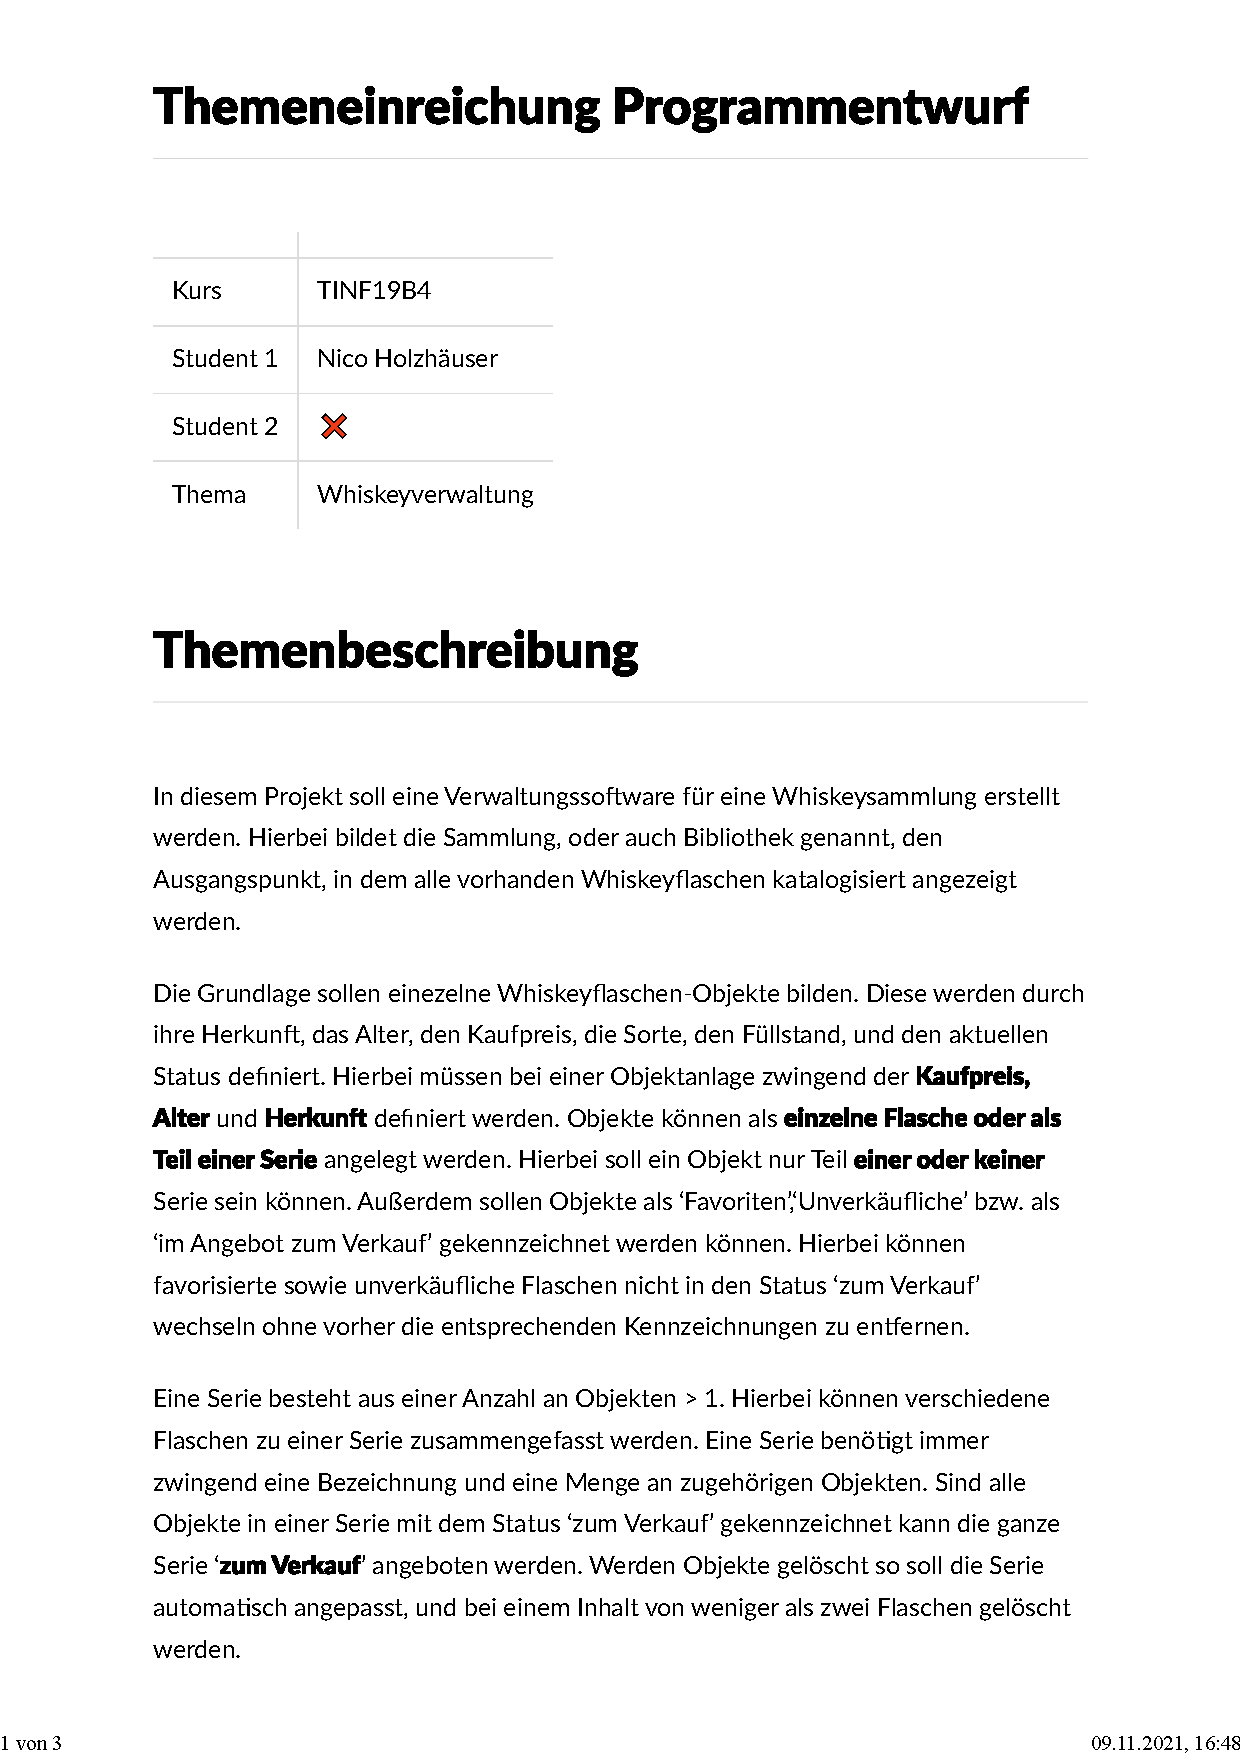
\includegraphics[scale=0.34,page=1]{./zfiles/Dokumente/ThemeneinreichungProgrammentwurf.pdf}}
		\frame{\includegraphics[scale=0.34,page=2]{./zfiles/Dokumente/ThemeneinreichungProgrammentwurf.pdf}}
		\frame{\includegraphics[scale=0.34,page=3]{./zfiles/Dokumente/ThemeneinreichungProgrammentwurf.pdf}}
	\end{landscape}
\end{center}

	%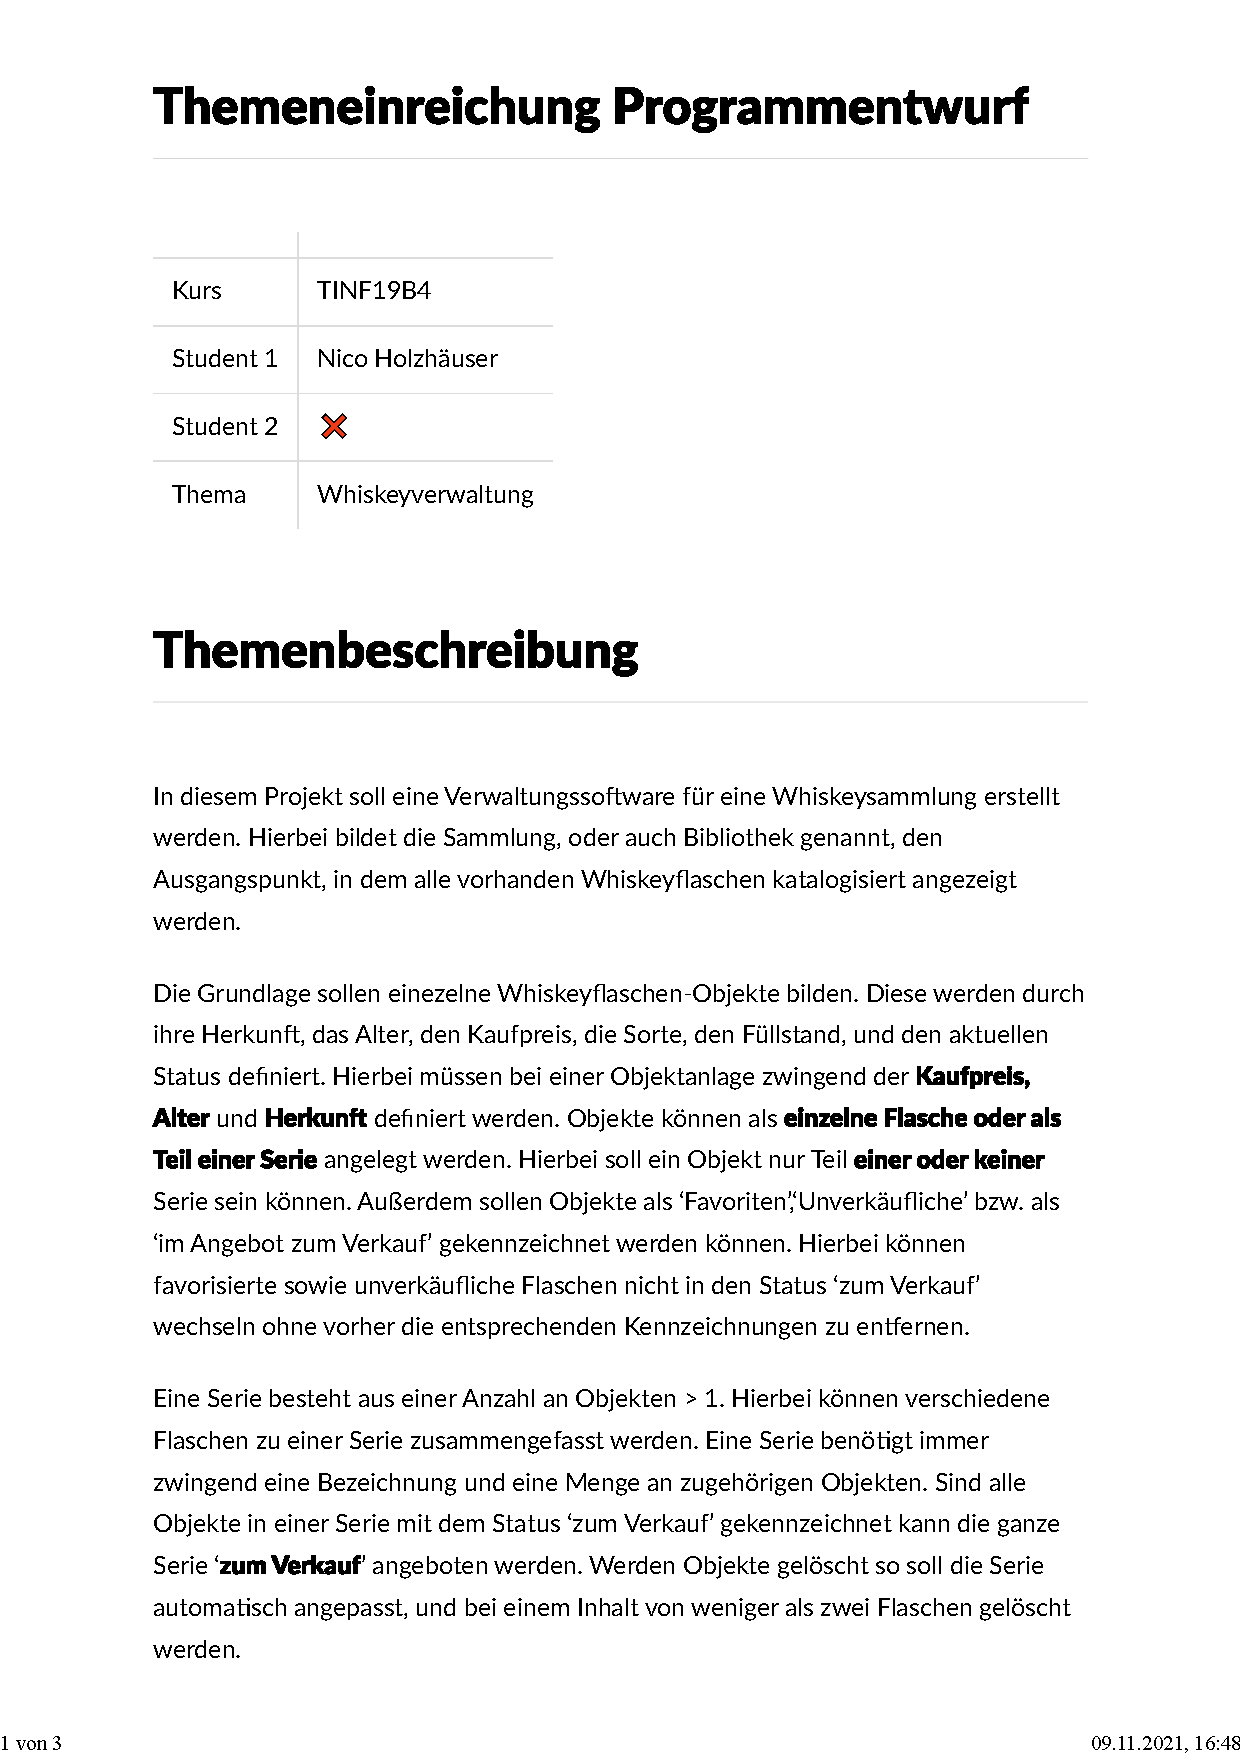
\includepdf[pages={1-3}]{./zfiles/Dokumente/ThemeneinreichungProgrammentwurf.pdf}
%======================================================================
%	
%	                _                       
%	    /\         | |                      
%	   /  \   _ __ | |__   __ _ _ __   __ _ 
%	  / /\ \ | '_ \| '_ \ / _` | '_ \ / _` |
%	 / ____ \| | | | | | | (_| | | | | (_| |
%	/_/    \_\_| |_|_| |_|\__,_|_| |_|\__, |
%								       __/ |
%									  |___/ 
%
%----------------------------------------------------------------------
% Descripton : Appendix 1
%======================================================================

\section{Aggregate Visualisierung} \label{a.1.aggregate}
	\begin{figure}[h]
		\centering
		%\includegraphics[height=150px]{./appendix/filesONLYForAppendix/Images/lion.png}
		\shadowimage[height=250px]{./zfiles/Bilder/aggregate.png}
		\caption{Aggregate Visualisierung \cite{domainModell.microsoft}}
		\label{a.1.aggregate}
	\end{figure}

\newpage

\section{\acl{DDD} Visualisierung} \label{a.1.ddd}
	\begin{figure}[h]
		\centering
		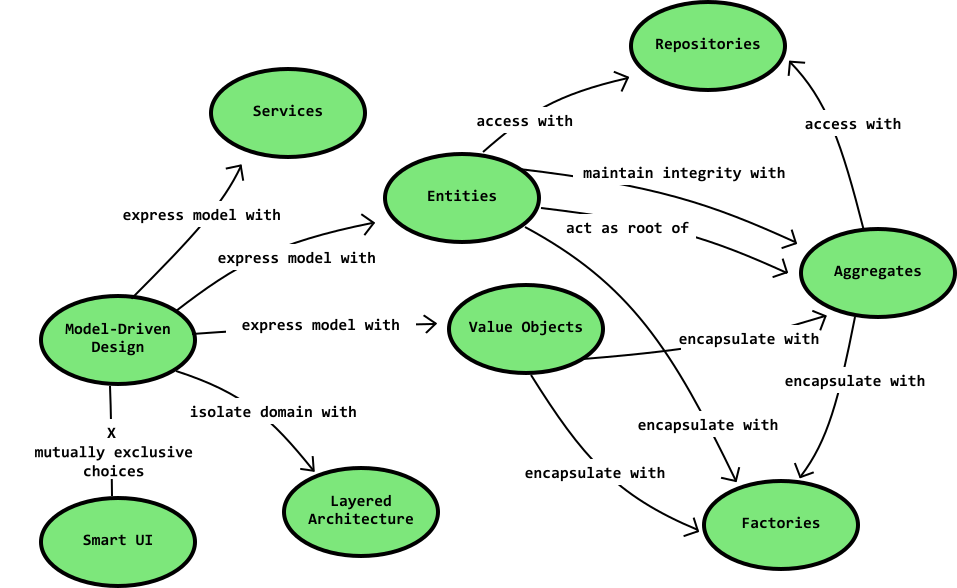
\includegraphics[height=250px]{./zfiles/Bilder/ddd.png}
		%\shadowimage[height=250px]{./zfiles/Bilder/ddd.png}
		\caption{\acl{DDD} Visualisierung \cite{ddd.stemmler}}
		\label{a.1.ddd}
	\end{figure}

\newpage

%======================================================================
%	
%	                _                       
%	    /\         | |                      
%	   /  \   _ __ | |__   __ _ _ __   __ _ 
%	  / /\ \ | '_ \| '_ \ / _` | '_ \ / _` |
%	 / ____ \| | | | | | | (_| | | | | (_| |
%	/_/    \_\_| |_|_| |_|\__,_|_| |_|\__, |
%								       __/ |
%									  |___/ 
%
%----------------------------------------------------------------------
% Descripton : Appendix 2
%======================================================================

\section{Clean Architecuture in Spring Boot} \label{a.2.cleanArchitecture}
\begin{figure}[h]
	\centering
	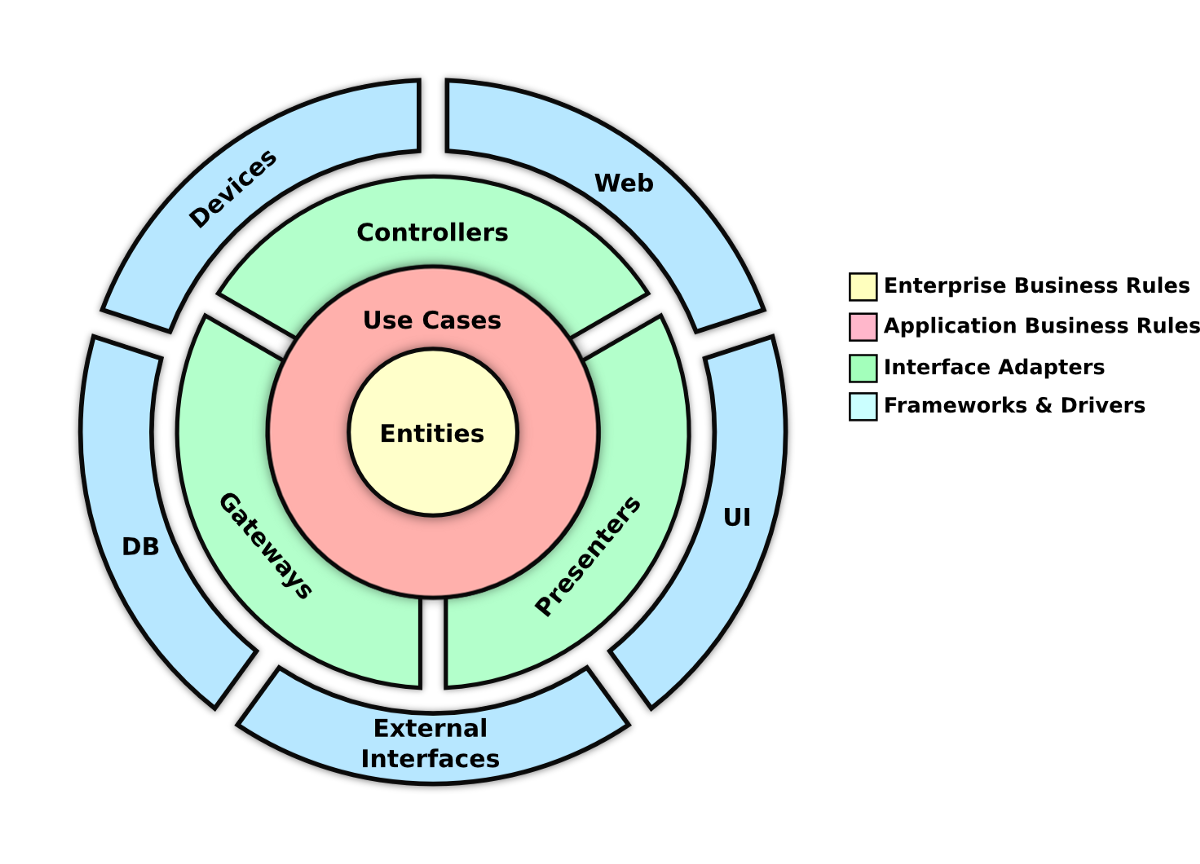
\includegraphics[height=350px]{./zfiles/Bilder/cleanArchitecture.png}
	%\shadowimage[height=250px]{./zfiles/Bilder/cleanArchitecture.png}
	\caption{Clean Architecuture in Spring Boot \cite{cleanArchitecture.medium}}
	\label{a.2.cleanArchitecture}
\end{figure}

\newpage
\input{./appendix/chapters/appendixChapter3.tex}
%======================================================================
%	
%	                _                       
%	    /\         | |                      
%	   /  \   _ __ | |__   __ _ _ __   __ _ 
%	  / /\ \ | '_ \| '_ \ / _` | '_ \ / _` |
%	 / ____ \| | | | | | | (_| | | | | (_| |
%	/_/    \_\_| |_|_| |_|\__,_|_| |_|\__, |
%								       __/ |
%									  |___/ 
%
%----------------------------------------------------------------------
% Descripton : Appendix 4
%======================================================================
\section{Code Smell - Backend - 1 - Before} \label{a.4.backend.codesmell1.before}
\begin{figure}[h]
	\centering
	%\includegraphics[height=150px]{./appendix/filesONLYForAppendix/Images/lion.png}
	\shadowimage[height=190px]{./zfiles/Bilder/BeforeRefactoringBackend.png}
	\caption{Code Smell - Backend - 1 - Before}
	\label{a.1.aggregate}
\end{figure}

\section{Code Smell - Backend - 1 - Fix} \label{a.4.backend.codesmell1.fix}
\begin{figure}[h]
	\centering
	%\includegraphics[height=150px]{./appendix/filesONLYForAppendix/Images/lion.png}
	\shadowimage[height=190px]{./zfiles/Bilder/BeforeRefactoringBackendCleanup.png}
	\caption{Code Smell - Backend - 1 - Fix}
	\label{a.1.aggregate}
\end{figure}

\newpage

\section{Code Smell - Backend - 1 - After} \label{a.4.backend.codesmell1.after}
\begin{figure}[h]
	\centering
	%\includegraphics[height=150px]{./appendix/filesONLYForAppendix/Images/lion.png}
	\shadowimage[height=190px]{./zfiles/Bilder/AfterRefactoringBackend.png}
	\caption{Code Smell - Backend - 1 - After}
	\label{a.1.aggregate}
\end{figure}

\newpage

\section{Code Smell - Backend - 2 - Before} \label{a.4.backend.codesmell2.before}
\begin{figure}[h]
	\centering
	%\includegraphics[height=150px]{./appendix/filesONLYForAppendix/Images/lion.png}
	\shadowimage[height=190px]{./zfiles/Bilder/BeforeRefactoringBackendPrimitivew.png}
	\caption{Code Smell - Backend - 2 - Before}
	\label{a.1.aggregate}
\end{figure}

\section{Code Smell - Backend - 2 - After} \label{a.4.backend.codesmell2.after}
\begin{figure}[h]
	\centering
	%\includegraphics[height=150px]{./appendix/filesONLYForAppendix/Images/lion.png}
	\shadowimage[height=190px]{./zfiles/Bilder/AfterRefactoringBackendBoolean.png}
	\caption{Code Smell - Backend - 2 - After}
	\label{a.1.aggregate}
\end{figure}

\newpage

\section{Code Smell - Frontend - 1 - Before} \label{a.4.frontend.codesmell1.before}
\begin{figure}[h]
	\centering
	%\includegraphics[height=150px]{./appendix/filesONLYForAppendix/Images/lion.png}
	\shadowimage[height=190px]{./zfiles/Bilder/BeforeRefactoringFrontend.png}
	\caption{Code Smell - Backend - 1 - Before}
	\label{a.1.aggregate}
\end{figure}

\section{Code Smell - Frontend - 1 - After} \label{a.4.frontend.codesmell1.after}
\begin{figure}[h]
	\centering
	%\includegraphics[height=150px]{./appendix/filesONLYForAppendix/Images/lion.png}
	\shadowimage[height=190px]{./zfiles/Bilder/AfterRefactoringFrontend.png}
	\caption{Code Smell - Backend - 1 - Fix}
	\label{a.1.aggregate}
\end{figure}

\newpage

%======================================================================
%	
%	                _                       
%	    /\         | |                      
%	   /  \   _ __ | |__   __ _ _ __   __ _ 
%	  / /\ \ | '_ \| '_ \ / _` | '_ \ / _` |
%	 / ____ \| | | | | | | (_| | | | | (_| |
%	/_/    \_\_| |_|_| |_|\__,_|_| |_|\__, |
%								       __/ |
%									  |___/ 
%
%----------------------------------------------------------------------
% Descripton : Appendix 5
%======================================================================
\section{Entwurfsmuster - Bridge - Before} \label{a.5.bridge.before}
\begin{figure}[h]
	\centering
	%\includegraphics[height=150px]{./appendix/filesONLYForAppendix/Images/lion.png}
	\shadowimage[height=350px]{./zfiles/Bilder/BeforeBridge.png}
	\caption{Entwurfsmuster - Bridge - Before}
	\label{a.1.aggregate}
\end{figure}

\newpage

\section{Entwurfsmuster - Bridge - After} \label{a.5.bridge.after}
\begin{figure}[h]
	\centering
	%\includegraphics[height=150px]{./appendix/filesONLYForAppendix/Images/lion.png}
	\shadowimage[height=325px]{./zfiles/Bilder/BridgeAfter.png}
	\caption{Entwurfsmuster - Bridge - After}
	\label{a.1.aggregate}
\end{figure}
	\cleardoublepage
	\ifthenelse{\boolean{DEBUG}}{}{\cleardoublepage}
	
	%—————————————————————————————————————————————————————————————————————————
	%						Literaturverzeichnis
	%—————————————————————————————————————————————————————————————————————————
	\renewcommand\bibname{Literaturverzeichnis \\ \vspace{10mm} \normalsize{} Alle Quellen sind zusätzlich im Ordner \HREF{./Quellensicherung}{Quellensicherung} gespeichert ! \vspace{-2cm}}
	\phantomsection
	\addcontentsline{toc}{chapter}{Literaturverzeichnis}
	\printbibliography
	\ifthenelse{\boolean{DEBUG}}{}{\cleardoublepage}
	
\end{document}